\section{Модел с репелент}
\begin{frame}[t]{Модел с репелент на Rashkov}
  По същността си уравненията на модела са като на Ross, но с усложнението, че може с помощта на репеленти да се намали честотата на ухапвания, тоест има множител $(1 - \kappa u(t))$ в закона за действие на масите, където $\kappa$ е ефективността на репелента, а пък $u(t)$ функция управление, задаващо пропорцията на хора предпазени с помощта на репелента.

  \begin{equation}
    \label{eq:RepelentProblem}
    \begin{split}
      &\dot{X}(t) = \beta_{vh} e^{-\mu \tau} a (1-\kappa u(t)) \frac{N-X(t)}{N} Y(t) - \gamma X(t) \\
      &\dot{Y}(t) = \beta_{hv} a (1-\kappa u(t)) X(t) (M-Y(t)) - \mu Y(t) \\
      &u(t) \in \mathscr{U} = \{u:\mathbb{R}_+ \rightarrow [0, \bar{u}] \vert u \text{- измерима}\}
    \end{split}
  \end{equation}

  $\tau$ е инкубационният период на комарите. Така математическото очакване заразèн комар да е станал зарàзен може да се изрази като $e^{-\frac{\tau}{\text{ср. продължителност на живот}}}$. Но средната продължителност на живот на комарите е точно $\frac{1}{\mu}$, откъдето $e^{-\mu\tau}Y$ е броя зарàзни комари.
\end{frame}

\begin{frame}[t]{Модел с репелент на Rashkov}
  Може да направим смяна от брой към пропорция на заразени. Така модела изглежда:
  \begin{equation}
    \begin{split}
      &\dot{x}(t) = \beta_{vh} e^{-\mu \tau} a \frac{M}{N} (1-\kappa u(t)) y(t) - \gamma x(t) \\
      &\dot{y}(t) = \beta_{hv} a (1-\kappa u(t)) x(t) (M-Y(t)) - \mu y(t) \\
      &u(t) \in \mathscr{U} = \{u:\mathbb{R}_+ \rightarrow [0, \bar{u}] \vert u \text{- измерима}\}
    \end{split}
  \end{equation}
  Надолу ще се пише и $z=(x,y)$
  Разглежда се следния казус - възможно ли е всички заразени да бъдат хоспитализирани, т.е. да са под $\bar{I}$?
  Въвеждаме $\mathfrak{I}(\bar{I}) = [0, \bar{I}] \cross [0, 1]$.
  Дефинира се ядрото на слаба инвариантност на Белман:
  $V(\bar{I}, \bar{u}) = \{z_0=(x_0, y_0) \vert \exists{u \in \mathscr{U}}\forall t>0 \left(x(t) < \bar{I}\right)\}$
\end{frame}

\begin{frame}[t]{Модел с репелент на Rashkov}
  Ако заместим с $\bar{u}$ получаваме автономна система и да се намерят равновесните ѝ точки.
  Ако $E^* = (x^*, y^*)$ е ендемична с $x^* > \bar{I}$, то $V(\bar{I}, \bar{u}) = \emptyset$, понеже може да се докаже, че е асимптотично устойчива.

  Може да се покаже, че ако $\bar{I} > \frac{(1-\kappa \bar{u}) \beta_{vh} e^{-\mu \tau} a \frac{M}{N}}{(1-\kappa \bar{u}) \beta_{vh} e^{-\mu \tau} a \frac{M}{N} + \gamma}$, то $V(\bar{I}, \bar{u}) = \mathfrak{I}(\bar{I})$.

  Как да подходим за другите стойности на $\bar{I}$?
\end{frame}

\begin{frame}[t]{Вариационна задача}
  Дефинираме значна фунцкия на разстоянието $\Gamma$ до границата на $\mathfrak{I}(\bar{I})$:
  \begin{equation}
    \Gamma(z) =
    \begin{cases}
      \inf_{z' \in \mathfrak{I}(\bar{I})} |z-z'|, \quad z \in \Omega \setminus \mathfrak{I}(\bar{I}) \\
      -\inf_{z' \in \Omega \setminus \mathfrak{I}(\bar{I})} |z-z'|, \quad z \in \mathfrak{I}(\bar{I})
    \end{cases}
  \end{equation}

  Фиксираме $l>L>0$ ($L$ - константата на Липшитц за системата) и въвеждаме функция на оценката $v$:
  \begin{equation}
    v(z_0) = \inf_{u \in \mathscr{U}} \sup_{t \in (0, +\infty)} e^{-lt} \Gamma(z(t; z_0; u))
  \end{equation}

  Ако започнем с $z_0 \notin V(\bar{I}, \bar{u})$, то $v(z_0) > 0$ и обратното.

  Ако започнем с $z_0 \in V(\bar{I}, \bar{u})$, то $v(z_0) \leq 0$ и обратното.

  Така $V(\bar{I}, \bar{u}) = \{z_0 \in \Omega \vert v(z) \leq 0\}$
\end{frame}

\begin{frame}[t]{Уравнение на Хамилтон-Якоби-Белман}
  Може да се покаже, че е изпълнено:
  \begin{equation}
    v(z_0) = \inf_{u \in \mathscr{U}} \max\{e^{-lt} v(z_0), \sup_{s \in (0, t]} e^{-lt} \Gamma(z(s; z_0; u))\}
  \end{equation}
  Може да се покаже, че $v$ е точно решението на:
  \begin{equation}
    \begin{split}
      &\min\{l v(z) + \max_{u \in \mathscr{U}} \mathcal{H}(z, u, \grad{v}), v(z) - \Gamma(z) \} = 0, \quad z \in \mathbb{R}^2 \\
      &\mathcal{H}(z, u, \grad{v}) = \innerproduct{-f(z, u)}{\grad{v}}
    \end{split}
  \end{equation}
  Диференциалното уравнение се разглежда като стационарно решение на диференцална задача, включваща време.
  За решаване на задачи от този вид има методи WENO (Weighted Essentially Non-Oscillatory) от с голяма точност, които апроксимират решението.
\end{frame}

\begin{frame}[t]{Резултати на Rashkov}
  \begin{figure}
    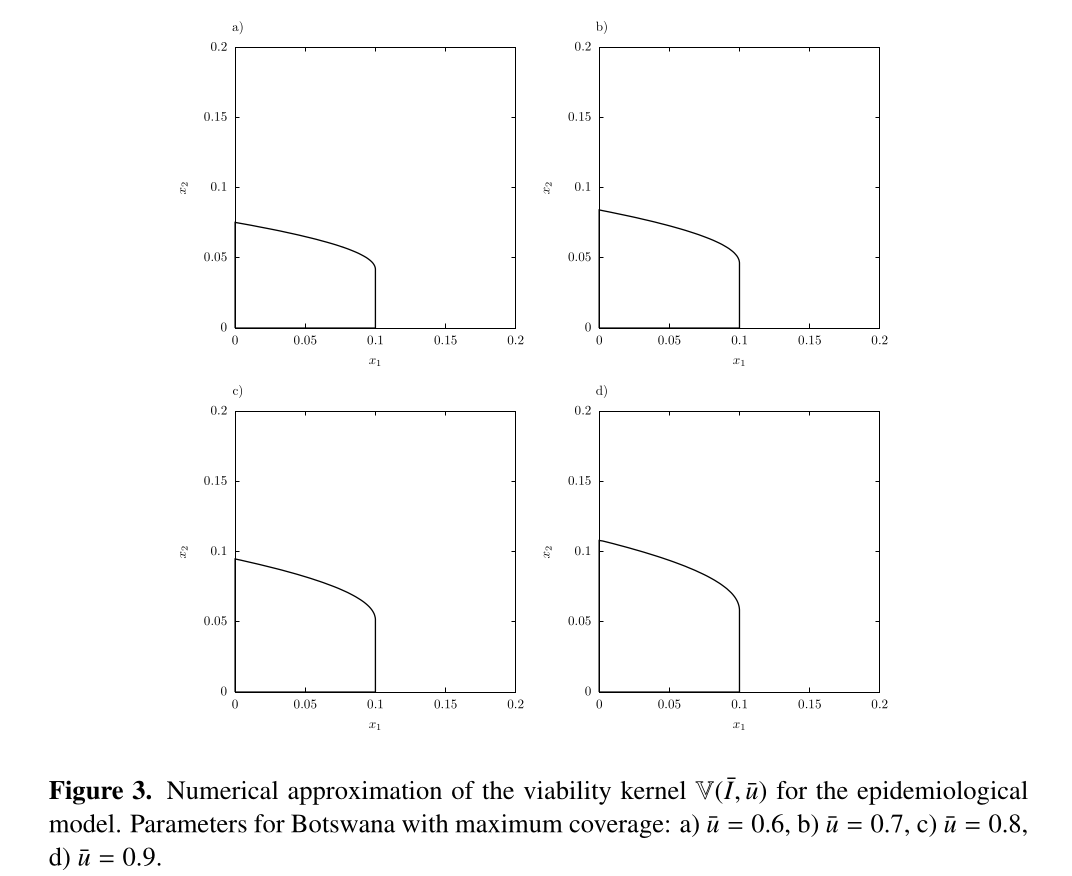
\includegraphics[width=0.7\paperwidth, height=0.8\paperheight]{rashkov-results.png}
  \end{figure}
\end{frame}
